%!TeX program = xelatex
\documentclass[12pt,a4paper,UTF8]{ctexart}

\usepackage[left=2.5cm,right=2.5cm,top=2.5cm,bottom=2.5cm]{geometry}
\usepackage{amsmath,amssymb}
\usepackage{booktabs}
\usepackage{graphicx}
\usepackage{float}
\usepackage{tabularx}
\usepackage{array}
\usepackage{xcolor}
\usepackage{listings}
\usepackage{hyperref}
\usepackage{fancyhdr}
\usepackage{longtable}
\usepackage{caption}
\usepackage{subcaption}

\graphicspath{{figures/}}
\hypersetup{colorlinks=true,linkcolor=black,urlcolor=blue,citecolor=blue}
\setlength{\headheight}{15pt}
\setlength{\emergencystretch}{3em}
\pagestyle{fancy}
\fancyhead[L]{信息安全技术}
\fancyhead[C]{期末课程报告}
\fancyhead[R]{大语言模型文本水印}

\lstset{
    basicstyle=\ttfamily\small,
    breaklines=true,
    frame=single,
    columns=fullflexible,
    keepspaces=true
}

\newcommand{\method}{CA-KL}
\newcommand{\fullmethod}{CA-KL-CG}
\newcommand{\codepath}[1]{\nolinkurl{#1}}

\begin{document}

\begin{titlepage}
    \centering
    \vspace*{1.2cm}
    
\includegraphics[width=0.48\textwidth]{sysu.jpg}
    \vspace{1.8cm}

    {\zihao{2}\heiti 信息安全技术课程期末报告\par}
    \vspace{1.1cm}
    {\zihao{3}\heiti 基于 KL 约束与加权检测的大语言模型文本水印改进研究\par}
    \vspace{0.5cm}
    {\zihao{4} 基于 ICML 2023 论文 \textit{A Watermark for Large Language Models} 的复现与改进\par}

    \vfill
    \begin{tabular}{rl}
        学生姓名： & 施煌，祖裕柏，黄镇邦 \\
        学号： & 23336204，23344188，23342035 \\
        院系： & 计算机学院 \\
    \end{tabular}
    \vfill
    {\large 2026 年 7 月}
\end{titlepage}

\begin{abstract}
本报告围绕大语言模型生成文本的溯源问题展开。我们选择 ICML 2023 论文 \textit{A Watermark for Large Language Models} 作为复现对象，先完成了原始 KGW 文本水印方法的代码运行、批量实验和统计检测，再在固定水印强度的局限上继续改进。最初我们尝试过基于熵的自适应 \texttt{delta}，它能解释为在高不确定位置增强水印、在低不确定位置减弱水印，但实验和进一步阅读文献让我们意识到，仅把熵线性映射为偏置强度仍然偏经验化，检测端也没有跟生成端形成闭环。

在最终方案中，我们提出并实现了 \method{} Watermark：每一步生成时不再直接指定固定 \texttt{delta}，而是在 KL 散度预算约束下选择最大可用水印偏置，使加水印后的分布 $P'_t$ 不会过度偏离原始模型分布 $P_t$。在检测端，我们进一步实现了模型辅助的 entropy-weighted detector 和 windowed detector，使检测统计量更关注高熵、可嵌入性更强的位置。实验使用 \texttt{facebook/opt-2.7b} 模型和 C4/realnewslike 数据集, 结果显示，\method{} 的检测成功率达到 96\%，高于 \texttt{Fixed Delta 2.0} 和自适应 \texttt{delta} 的 91\%；同时 \method{} 的 Distinct-1 为 0.7057、重复率为 0.2943，均优于强水印 \texttt{Fixed Delta 3.0}。这说明本文方法在检测能力和文本质量之间取得了比固定强水印更合理的折中。

\noindent\textbf{关键词：}大语言模型；文本水印；信息安全；KL 散度；加权检测；内容溯源
\end{abstract}

\clearpage
\pagenumbering{Roman}
\tableofcontents
\clearpage
\pagenumbering{arabic}

\section{引言}

大语言模型在内容生成、问答辅助、教育支持、编程协作等场景中已经表现出很强的实用价值，但与此同时，模型输出内容的可追踪性与可验证性问题也逐渐成为信息安全领域的重要研究方向。一方面，大模型生成文本在形式上越来越接近人工撰写内容，如果缺少额外标记，平台、教师、企业和监管者很难快速判断某段文本是否由模型生成；另一方面，生成式模型被广泛接入搜索、写作和社交平台之后，伪造信息、自动批量灌水、学术不端和内容归属不清等问题也更加突出。在这样的背景下，文本水印技术成为连接生成模型与内容治理的重要安全机制。与传统密码学中的加密或签名不同，文本水印不要求直接暴露密钥，也不要求改变文本的外部显示格式，而是通过对生成过程施加概率偏置，使得文本在统计意义上带有可检测的“生成痕迹”。因此，围绕文本水印开展复现和改进，不仅契合《信息安全技术》课程中关于数字水印的主题，也具有很强的现实应用价值。

我们复现的原始论文是 Kirchenbauer 等人在 ICML 2023 发表的 \textit{A Watermark for Large Language Models}~\cite{kirchenbauer2023watermark}。这篇论文提出的 KGW 方法思路清楚、代码开源，适合作为课程大作业的基础。它在每一步生成前，根据已有上下文用伪随机方式把词表划分为 greenlist 和 redlist，然后给 greenlist 中的 token logits 加上固定偏置 \texttt{delta}。检测时只要用同样的密钥和上下文重建 greenlist，再统计文本中 green token 的数量是否异常偏高，就可以判断文本是否可能由带水印模型生成。

在继续改进前，我们还阅读了后续关于水印可靠性和自适应水印的工作。可靠性研究提醒我们，水印检测不能只依赖一个漂亮的阈值数字，还要关注误报率、文本长度、攻击和统计校准等因素~\cite{kirchenbauer2024reliability}；自适应水印方向则说明，不同生成位置的可嵌入性确实不同，熵和模型置信度可以作为调节水印强度的重要信号~\cite{liu2024adaptive}。这两点共同影响了我们的最终设计：生成端用 KL 预算约束扰动，检测端用加权和校准指标重新评价水印证据。

刚开始复现时，我们觉得固定 \texttt{delta} 已经足够直接：偏置越大，green token 越多，检测越容易。但真正跑完不同 \texttt{delta} 的对比后，我们发现强水印确实能把 z-score 推高，但同时也会更明显地干预模型原本的选择，使文本多样性下降、重复率上升。这个观察把我们的改进方向从单纯追求检测率拉回到了更合理的问题：怎样在不明显破坏原始生成分布的情况下，尽量留下稳定的水印证据。

因此，本报告的改进目标不是简单超过所有固定 \texttt{delta} 设置，而是希望提出一种更可解释的质量--检测折中机制。我们最终采用 KL 散度作为每一步分布扰动的预算，并配合加权检测器重新评估水印信号。这个过程也改变了我们对文本水印的理解：水印强度本身不是孤立参数，它应该和当前位置的模型分布、可嵌入性以及检测统计量一起设计。

\section{原论文方法阅读与复现}

\subsection{KGW 文本水印的基本机制}

KGW 方法的核心是 seeded greenlist。设词表大小为 $|\mathcal{V}|$，水印参数 $\gamma$ 控制 greenlist 占词表的比例。对于当前前缀 $x_{<t}$，算法用密钥和前缀生成伪随机种子，再由该种子把词表划分为 greenlist $G_t$ 和 redlist $R_t$。如果模型原始输出 logits 为 $l_t(v)$，水印生成器会对 $v\in G_t$ 的 token 加上固定偏置：
\[
l'_t(v)=
\begin{cases}
l_t(v)+\delta, & v\in G_t,\\
l_t(v), & v\notin G_t.
\end{cases}
\]
随后模型根据修改后的分布进行采样。这样生成出的文本不会在表面出现特殊符号，但 green token 的出现比例会高于自然文本。

检测端使用同样的种子规则逐 token 重建 greenlist，并统计生成文本中落入 greenlist 的 token 个数。假设无水印文本中每个 token 落入 greenlist 的概率约为 $\gamma$，长度为 $T$ 的文本中 green token 的期望数量为 $\gamma T$，方差为 $T\gamma(1-\gamma)$。因此原论文使用 z-score 衡量偏离程度：
\[
z=\frac{|s|_G-\gamma T}{\sqrt{T\gamma(1-\gamma)}}.
\]
这里 $|s|_G$ 是观测到的 green token 数量。z-score 越高，说明文本中 green token 多得越不正常，也就越支持该文本带有水印。论文同时给出 $p$-value 和阈值判断，因此它本质上不是训练一个二分类器，而是在生成过程里嵌入一种可重复验证的统计偏差。

从代码结构上看，官方实现主要由两个类支撑。生成阶段的 \texttt{WatermarkLogitsProcessor} 继承 Hugging Face 的 \texttt{LogitsProcessor}，在每一步生成前根据当前 prefix 计算 greenlist，并给 greenlist token 加上固定 \texttt{delta}。检测阶段的 \texttt{WatermarkDetector} 按照同样的 seeding 规则重建 greenlist，输出 \texttt{num\_green\_tokens}、\texttt{green\_fraction}、\texttt{z\_score}、\texttt{p\_value} 和最终 \texttt{prediction}。我后续改进时一直保留这条主线，因为它让生成和检测之间存在清晰的密钥一致性。

\subsection{官方仓库与复现环境}

复现工作从官方仓库 \codepath{jwkirchenbauer/lm-watermarking} 开始。这个仓库包含 \codepath{demo_watermark.py}、\codepath{watermark_processor.py}、\codepath{extended_watermark_processor.py}、\codepath{normalizers.py} 和 \codepath{alternative_prf_schemes.py} 等核心文件，其中最关键的是 \codepath{watermark_processor.py}，它实现了基础 KGW 水印生成器和检测器。图~\ref{fig:official-repo} 是我复现时使用的官方仓库页面，后续课程代码也是在这个仓库结构上整理出来的。

\begin{figure}[H]
    \centering
    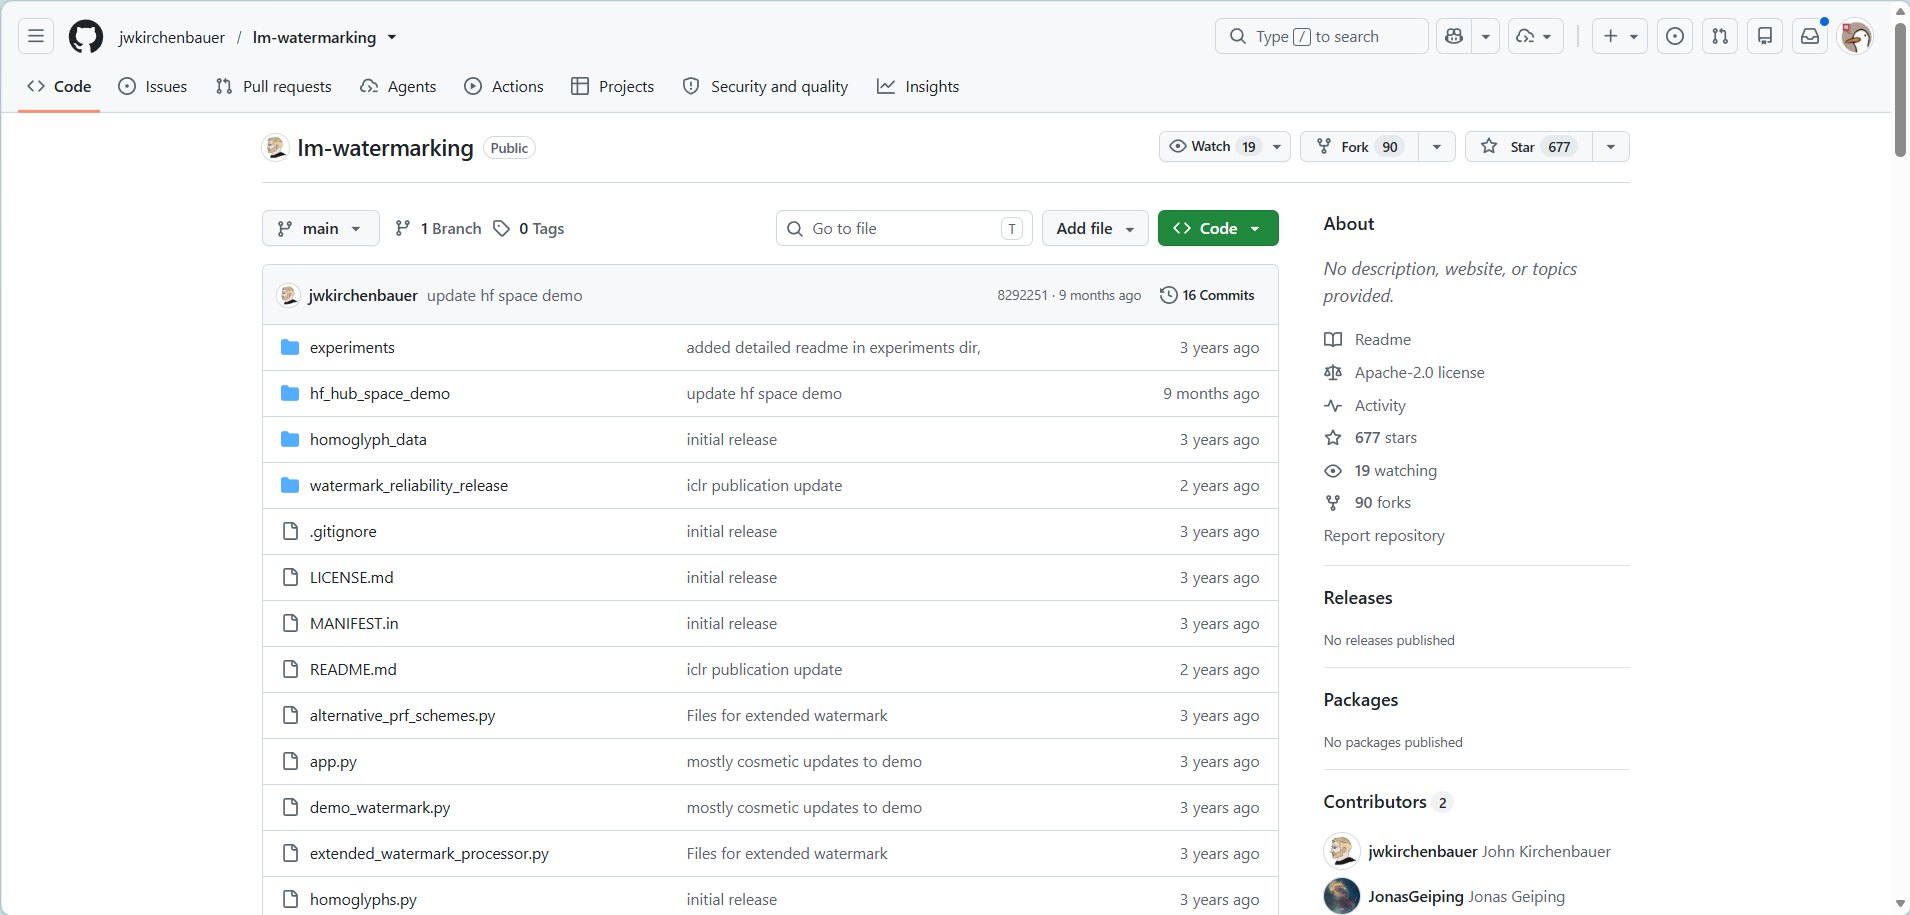
\includegraphics[width=0.92\textwidth]{official_repo.png}
    \caption{官方 lm-watermarking 仓库页面}
    \label{fig:official-repo}
\end{figure}

我们在本地 Windows + Anaconda 环境中完成复现与后续改进。正式实验环境使用 \texttt{pytorch} conda 环境，核心依赖包括 PyTorch、Transformers、datasets、scipy、pandas 和 matplotlib。模型方面，复现阶段先使用 \texttt{sshleifer/tiny-gpt2} 跑通官方 Demo，因为它下载快、显存压力小，适合排查环境和接口问题；确认生成、检测、CSV 输出和绘图流程没有问题后，再下载并使用 \texttt{facebook/opt-2.7b} 作为正式实验模型。

为了避免课程改进代码和原始复现代码互相污染，我们把新增内容集中放在 \codepath{course_project/} 目录下。其中 \codepath{processors/} 保存改进后的 logits processor 和 detector，\codepath{scripts/} 保存批量实验、prompt 准备和结果分析脚本，\codepath{outputs/} 保存 CSV、Markdown 摘要和图表。这样的组织方式对后续调参很有帮助，因为我们可以在不破坏原始 \codepath{watermark_processor.py} 的前提下，反复比较固定 \texttt{delta}、旧自适应方法和新方法。

\subsection{原始复现步骤}

官方复现按照“仓库准备、依赖安装、模型下载、Demo 启动、结果验证”的顺序完成。最初我们并没有直接运行大模型，而是先让最小模型把完整链路跑通，这一步能提前暴露 Gradio、Transformers 和本地模型路径的问题。核心命令如下：

\begin{lstlisting}[language=bash]
git clone https://github.com/jwkirchenbauer/lm-watermarking.git
cd lm-watermarking
conda create -n inform python=3.10 -y
conda activate inform
pip install -r requirements.txt
\end{lstlisting}

模型准备完成后，使用本地 tiny-gpt2 启动官方 Gradio Demo：

\begin{lstlisting}[language=bash]
python demo_watermark.py \
  --model_name_or_path ./models/tiny-gpt2 \
  --use_gpu True \
  --run_gradio True \
  --max_new_tokens 100
\end{lstlisting}

复现过程中遇到的一个实际问题是 Gradio 版本兼容。官方旧代码中使用的 \texttt{demo.queue(concurrency\_count=3)} 在新版 Gradio 中已经不再兼容，启动时会报参数错误。我们把它改为 \texttt{demo.queue(default\_concurrency\_limit=3)} 后，前端页面可以正常打开。这个修复本身不改变水印算法，只是让官方交互式 Demo 能在当前环境下运行。图~\ref{fig:official-demo-start} 展示了官方 Demo 正常启动后的界面。

\begin{figure}[H]
    \centering
    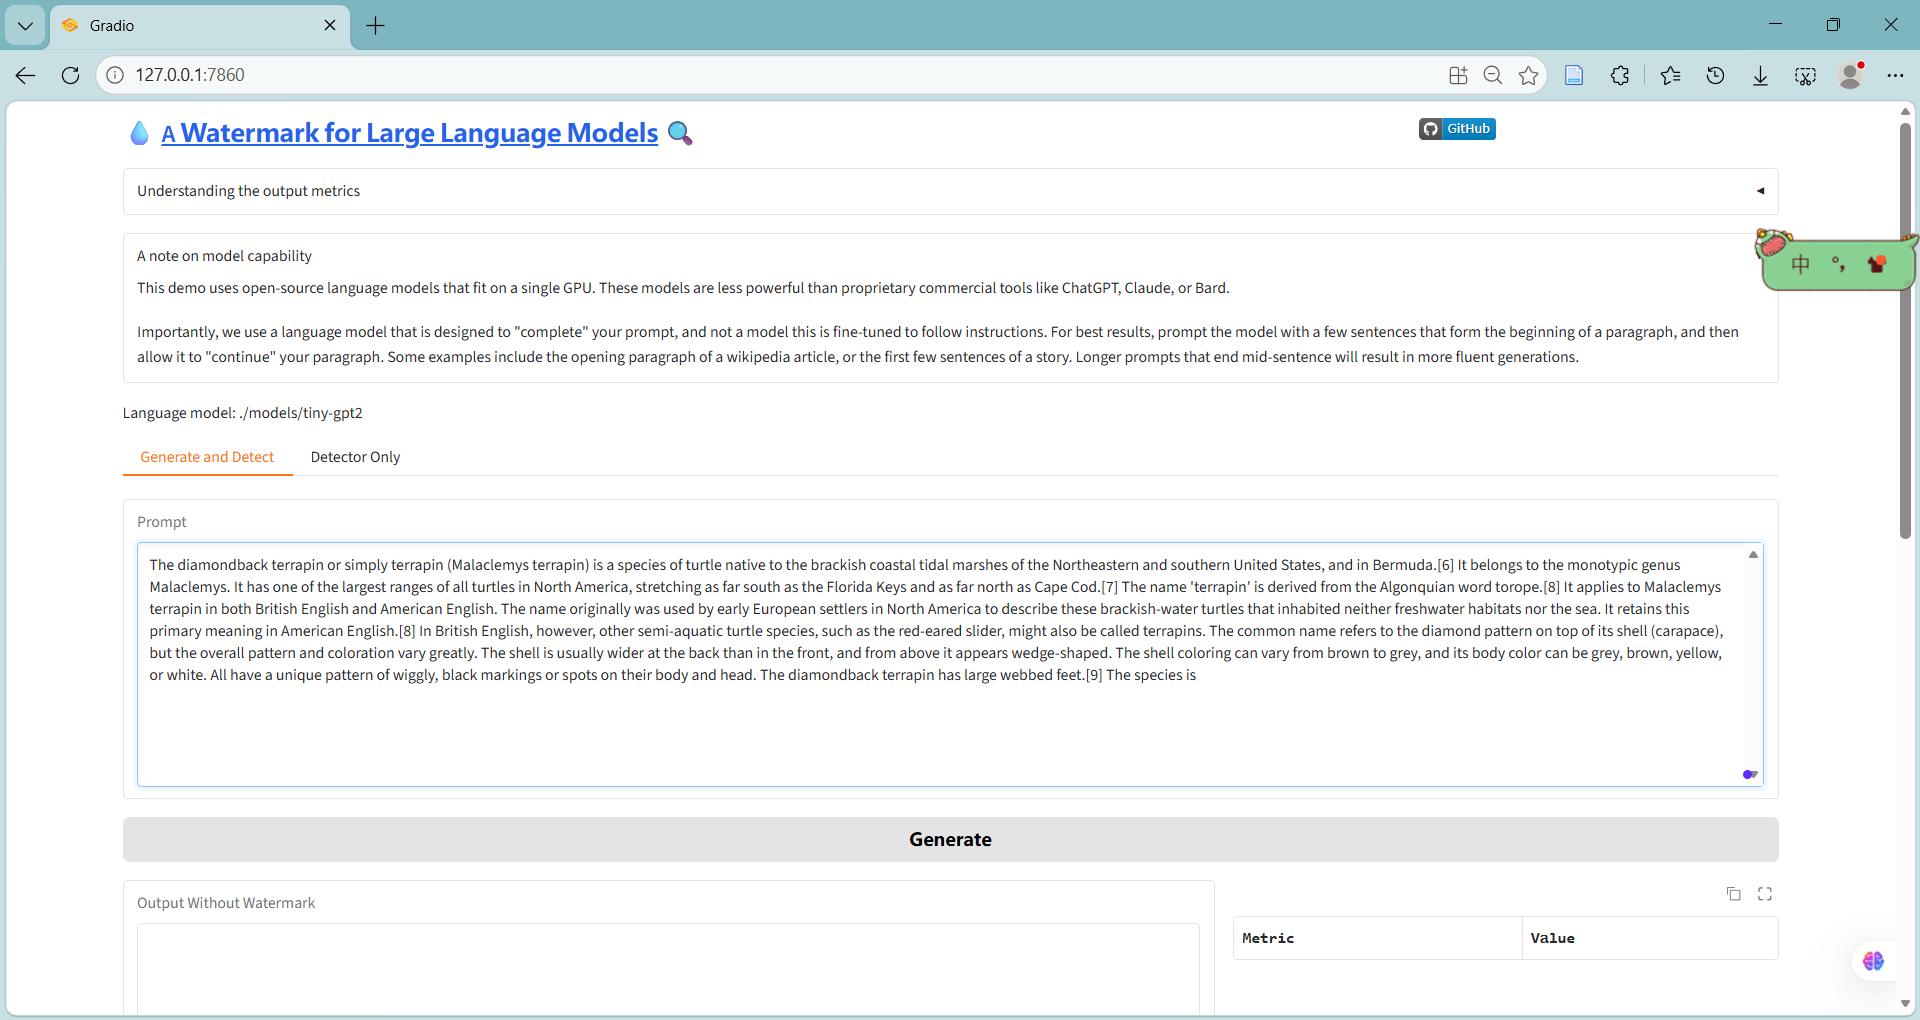
\includegraphics[width=0.92\textwidth]{official_demo_start.png}
    \caption{官方 Gradio Demo 启动界面}
    \label{fig:official-demo-start}
\end{figure}

\subsection{复现结果与验证}

官方 Demo 的验证方式很直接：输入同一个 prompt，系统同时生成无水印文本和带水印文本，并在右侧输出各自的检测统计量。一次典型复现结果如图~\ref{fig:official-demo-detection} 所示，无水印文本统计到 $T=99$ 个 token，其中 green token 数量为 22，\texttt{green\_fraction} 为 22.2\%，\texttt{z-score=-0.638}，检测结果为 \texttt{Human/Unwatermarked}；带水印文本统计到 $T=98$ 个 token，其中 green token 数量为 69，\texttt{green\_fraction} 为 70.4\%，\texttt{z-score=10.4}，检测结果为 \texttt{Watermarked}，置信度接近 100\%。

\begin{figure}[H]
    \centering
    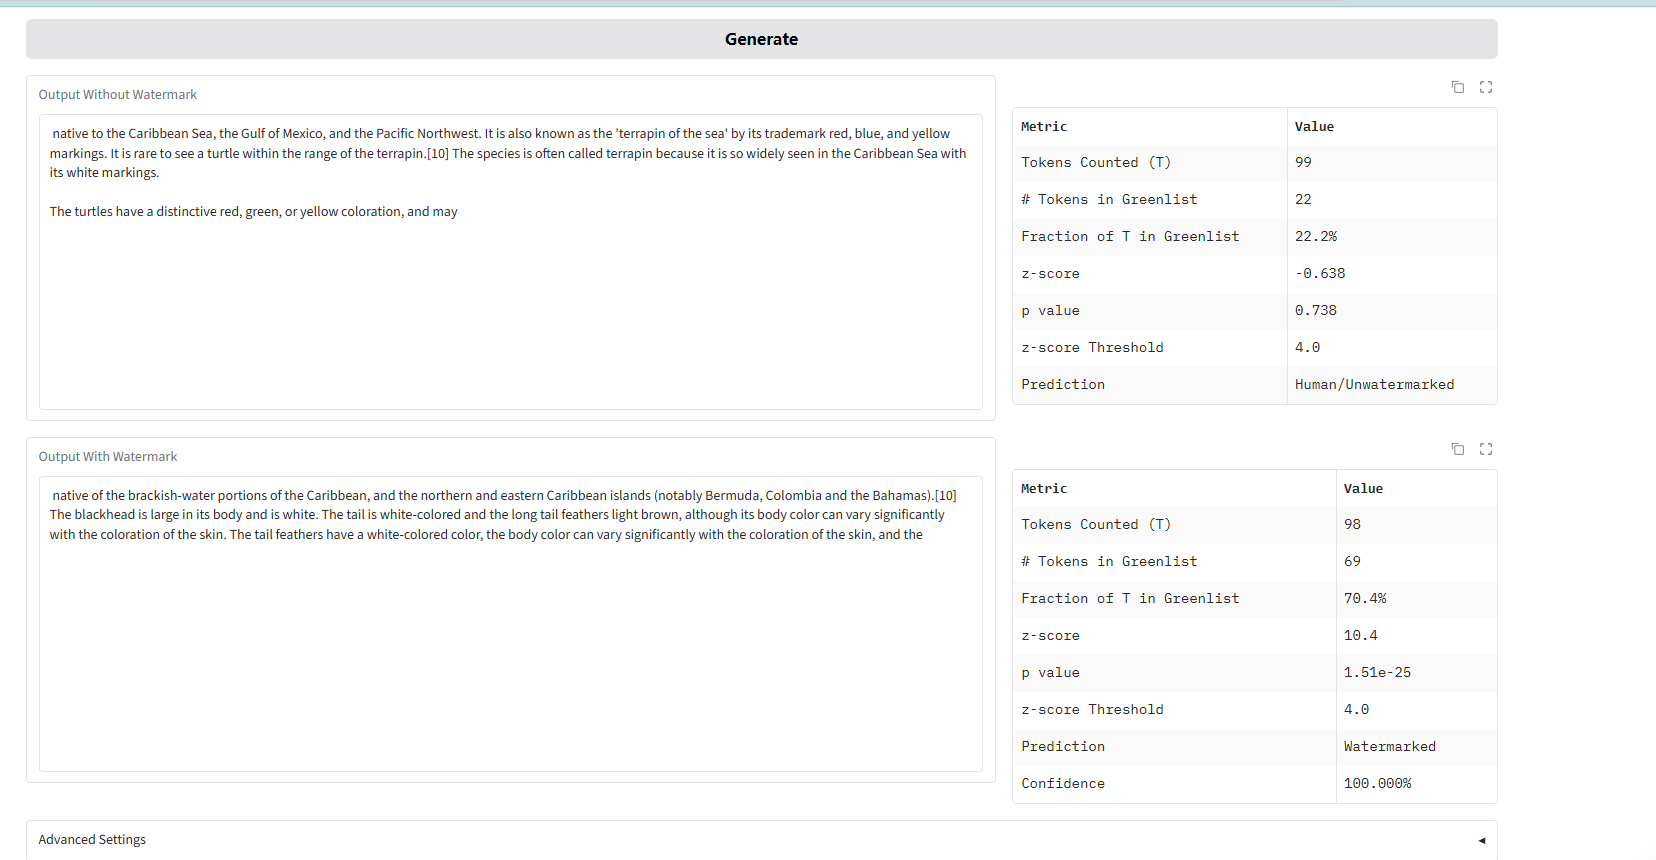
\includegraphics[width=0.92\textwidth]{official_demo_detection.png}
    \caption{官方 Demo 中无水印文本与带水印文本的检测结果}
    \label{fig:official-demo-detection}
\end{figure}

这个结果让我们对原论文方法有了更直观的理解。水印并不是在文本表面添加某个特殊符号，而是在生成概率里持续施加很小的统计倾向；单个 token 看起来仍然自然，但几十个 token 累积后，green token 占比会显著偏离自然文本。也正因为这一点，z-score 成为后续实验最重要的检测指标之一。

\subsection{复现中观察到的问题}

完成官方 Demo 复现后，我们进一步在批量脚本中比较了不同固定 \texttt{delta} 的效果。\texttt{delta} 越大，green fraction 和 z-score 越高，检测成功率也越高。但当我们观察质量指标时，强水印的代价也出现了。以最新 100 条 OPT-2.7B 实验为例，\texttt{Fixed Delta 3.0} 的检测成功率达到 100\%，平均 z-score 达到 10.2261，但 Distinct-1 只有 0.6879，Distinct-2 降到 0.8727，重复率升到 0.3121。相比之下，较弱的水印和后续自适应方法虽然检测分数低一些，却能保留更好的多样性。

这使我们意识到，固定 \texttt{delta} 的问题不在于它不能检测，而在于它把所有生成位置当成一样处理。有些位置模型本来就非常确定，例如固定搭配、常见虚词或标点附近，强行推动 green token 更容易伤害自然性；有些位置模型有多个合理候选，这时嵌入水印的代价更低。原始方法没有区分这种差异，这正是我们后续改进的切入点。

\section{从自适应方法到 CA-KL}

\subsection{ Adaptive Delta 的局限}

在第一版改进中，我们实现了基于熵的 Adaptive Delta。它的想法是先计算当前 next-token 分布的归一化熵 $H_{\text{norm}}$，再用经验函数把熵映射为当前步的水印强度：
\[
\delta_t=\delta_{\min}+(\delta_{\max}-\delta_{\min})\cdot f(H_{\text{norm}}).
\]
这个方法比固定 \texttt{delta} 更灵活，也容易解释：高熵位置有更多合理候选，适合更强水印；低熵位置更确定，应该更温和。

但我们后来发现，这个方法还不够像一个完整的改进。首先，熵到 \texttt{delta} 的映射本质上仍然是经验调参，我们很难说明为什么某个熵值就应该对应某个具体偏置。其次，检测器仍然是原始 KGW detector，生成端变了，检测端没有利用生成端记录的可嵌入性信息。

\subsection{使用 KL 约束重新定义水印强度}

我们最终把问题改写为一个受约束的选择问题：每一步不是先猜一个 \texttt{delta}，而是在可接受的分布扰动预算内，选择尽可能大的水印偏置。设原始模型分布为 $P_t$，加水印后的分布为 $P'_t$，本文要求：
\[
D_{\mathrm{KL}}(P'_t\|P_t)\leq \varepsilon.
\]
这个约束的含义是：水印可以改变模型分布，但这种改变不能超过预设预算 $\varepsilon$。在实现中，我们先计算当前 greenlist 在原始分布下的概率质量 $p_G$，再对 $\delta_t$ 做二分搜索。对于给定 $\delta$，归一化因子为：
\[
Z=1+(\exp(\delta)-1)p_G,
\]
加水印后 greenlist 的总概率质量为：
\[
q_G=\frac{\exp(\delta)p_G}{Z},
\]
对应的 KL 散度可以写成：
\[
D_{\mathrm{KL}}(P'_t\|P_t)=\delta q_G-\log Z.
\]
我们选择满足 KL 预算的最大 $\delta_t$。这样一来，水印强度不再是熵的线性变换，而是由当前分布和 KL 预算共同决定。实验中我们先尝试了 $\varepsilon=0.02$，结果发现平均 \texttt{delta} 过低，检测信号不足；经过 20 条 prompt 的网格实验后，我们选择 $\varepsilon=0.50$ 作为正式参数，此时 \method{} 的平均自适应 \texttt{delta} 为 2.4966，既足够形成水印痕迹，又仍然保留了分布约束的解释。

\subsection{加权检测器的作用}

在生成端引入自适应强度后，我们也重新考虑了检测端。原始 z-score 把每个 token 位置等权看待，但在我们的方法中，每个位置的可嵌入性并不一样。为了让检测器和生成器更一致，我们实现了模型辅助的 entropy-weighted detector。检测时，系统用同一个基础模型重新计算每个 prefix 的 logits，得到当前位置的熵、候选 greenlist 及其概率质量，并对高熵位置赋予更高权重。

加权检测的统计量为：
\[
Z_w=\frac{\sum_i w_i(G_i-p_i)}
{\sqrt{\sum_i w_i^2p_i(1-p_i)}}.
\]
其中 $G_i$ 表示第 $i$ 个生成 token 是否落入 greenlist，$p_i$ 是无水印条件下落入该 greenlist 的概率质量，$w_i$ 是由当前 prefix 分布计算出的权重。由于 $w_i$ 只依赖当前 token 之前的 prefix，不依赖当前 token 是否命中 greenlist，这个统计量在无水印文本下仍然有合理的零均值解释。

我们还实现了 windowed detector，即在多个窗口长度上计算局部加权 z-score，并取最大值。这个设计主要是为了后续处理 copy-paste 混入场景：如果一段带水印文本被插入到大量无水印文本中，全局统计量会被稀释，而窗口检测可以更容易发现局部水印片段。

\section{实现细节}

最终代码主要增加了三个部分。第一，\codepath{course_project/processors/cakl_watermark_processor.py} 中实现了 CA-KL 生成器，负责 KL-constrained adaptive delta、confidence gate 和 candidate-aware greenlist。第二，同一文件中实现了模型辅助检测器，负责 weighted z-score 和 WinMax weighted z-score。第三，\codepath{course_project/scripts/run_experiments.py} 被扩展为批量实验入口，可以一次性比较 \texttt{No Watermark}、多个固定 \texttt{delta}、旧 Adaptive Delta、\method{}、\method{} + Weighted Detector、Candidate Greenlist 和完整 \fullmethod{}。

我们在调试中保留了几个工程判断。首先，模型不做 fine-tuning，所有水印都在 inference-time 修改 logits，这使得项目规模可控，也更贴近原论文。其次，正式检测中采用模型辅助检测，这比原始 detector 慢，但能复现每个 prefix 下的分布状态，因而更适合评估自适应方法。最后，结果分析脚本不仅输出平均 z-score 和检测成功率，还会输出 AUC、TPR@1\%FPR、TPR@5\%FPR、平均 KL、平均自适应 \texttt{delta} 等诊断指标。

核心实验命令如下：
\begin{lstlisting}[language=bash]
python course_project/scripts/run_experiments.py \
  --model_name_or_path ./models/opt-2.7b \
  --prompt_source prompts_file \
  --prompts_path course_project/data/prompts_c4_realnewslike_500.txt \
  --output_csv course_project/outputs/cakl_opt27b_c4_100_eps050_results.csv \
  --max_new_tokens 100 \
  --use_gpu True \
  --load_fp16 True \
  --fixed_deltas 1.0 2.0 3.0 \
  --limit_prompts 100 \
  --run_cakl True \
  --kl_epsilon 0.50 \
  --cakl_delta_max 3.0 \
  --confidence_entropy_threshold 0.10 \
  --confidence_top1_threshold 0.95 \
  --candidate_top_p 0.95 \
  --use_model_assisted_detector True
\end{lstlisting}

\section{实验设置}

正式实验使用 \texttt{facebook/opt-2.7b}，该模型来自 OPT 开放预训练模型系列~\cite{zhang2022opt}。数据来自 C4/realnewslike，C4 本身是大规模清洗网页文本数据集~\cite{raffel2020exploring}。由于本地显存和时间有限，我们没有直接跑 500 条全量样本，而是在固定随机设置下选取前 100 条 prompt，每条最多生成 100 个 token。

\begin{table}[H]
    \centering
    \caption{正式实验设置}
    \label{tab:setup}
    \begin{tabularx}{0.92\textwidth}{p{0.30\textwidth}X}
        \toprule
        项目 & 设置 \\
        \midrule
        基础模型 & \texttt{facebook/opt-2.7b} \\
        数据集 & \texttt{C4/realnewslike}，保存为 \texttt{prompts\_c4\_realnewslike\_500.txt} \\
        正式评估样本数 & 100 条 prompt \\
        每条最大生成长度 & 100 tokens \\
        采样方式 & multinomial sampling，temperature = 0.7 \\
        水印比例参数 & $\gamma=0.25$ \\
        原始检测阈值 & z-score threshold = 4.0 \\
        \method{} 参数 & $\varepsilon=0.50$，\texttt{delta\_max=3.0} \\
        Confidence Gate & $H_{\text{norm}}\geq 0.10$，$p_{\text{top1}}\leq 0.95$ \\
        Candidate Greenlist & \texttt{top\_p=0.95} \\
        硬件 & NVIDIA GeForce RTX 5060 Laptop GPU，fp16 加载 \\
        \bottomrule
    \end{tabularx}
\end{table}

评价指标分为两类。第一类是原始 KGW 检测指标，包括 green fraction、z-score 和 detection success rate。第二类是文本质量与检测增强指标，包括 Distinct-1、Distinct-2、Repetition Rate、Weighted z-score、WinMax Weighted z-score、AUC 和 TPR@FPR。Distinct 越高通常说明文本越不重复，Repetition Rate 越低说明词汇重复越少。

\section{实验结果}

\subsection{主结果对比}

\begin{table}[H]
    \centering
    \caption{OPT-2.7B + C4/realnewslike 100 条样本主实验结果}
    \label{tab:main-results}
    \small
    \begin{tabularx}{\textwidth}{p{0.26\textwidth}rrrrrr}
        \toprule
        方法 & z-score & 检测率 & Green Frac. & Distinct-1 & Distinct-2 & 重复率 \\
        \midrule
        No Watermark & -0.3840 & 0\% & 0.2335 & 0.6946 & 0.9225 & 0.3054 \\
        Fixed Delta 1.0 & 2.8658 & 25\% & 0.3792 & 0.6942 & 0.9148 & 0.3058 \\
        Fixed Delta 2.0 & 6.6279 & 91\% & 0.5460 & 0.7002 & 0.9121 & 0.2998 \\
        Fixed Delta 3.0 & \textbf{10.2261} & \textbf{100\%} & \textbf{0.7096} & 0.6879 & 0.8727 & 0.3121 \\
        Current Adaptive Delta & 6.5619 & 91\% & 0.5433 & 0.6969 & 0.9062 & 0.3031 \\
        \method{} & 7.6077 & 96\% & 0.5927 & 0.7057 & 0.9073 & 0.2943 \\
        \method{} + Weighted Detector & 7.6077 & 96\% & 0.5927 & 0.7057 & 0.9073 & 0.2943 \\
        \fullmethod{} & 6.3767 & 87\% & 0.5408 & \textbf{0.7256} & \textbf{0.9257} & \textbf{0.2744} \\
        \bottomrule
    \end{tabularx}
\end{table}

从表 \ref{tab:main-results} 可以看到，\method{} 是这次实验中最适合作为主方案的结果。它的检测成功率为 96\%，高于 \texttt{Fixed Delta 2.0} 和 Current Adaptive Delta 的 91\%；平均 z-score 也从 6.6279 和 6.5619 提升到 7.6077。与此同时，\method{} 的 Distinct-1 为 0.7057，重复率为 0.2943，均优于强水印 \texttt{Fixed Delta 3.0}。这说明 KL 约束并没有让水印变得过弱，反而在保持可检测性的同时，避免了强固定偏置对文本质量的明显伤害。

\texttt{Fixed Delta 3.0} 的检测率仍然最高，这是合理的，因为它在每一步都用较大偏置强推 green token。问题在于，它的质量指标最差：Distinct-1 和 Distinct-2 均低于 \method{}，重复率高于 \method{}。我们在报告中不把它当成需要全面超过的对象，而是把它视为强水印上界，用来说明单纯提高检测强度会带来质量代价。

\fullmethod{} 的结果也很有意思。它的普通检测率只有 87\%，低于 \method{}，但它拥有最高的 Distinct-1 和 Distinct-2，以及最低的重复率。这说明 Candidate Greenlist 和 Confidence Gate 确实让生成过程更克制：它们减少了对不合适位置的干预，因此文本质量更好，但水印信号也相应变弱。我们会把 \fullmethod{} 定位为质量优先版本，而不是检测优先主方案。

\begin{figure}[H]
    \centering
    
\includegraphics[width=0.86\textwidth]{cakl_zscore.png}
    \caption{不同方法的平均 z-score 对比}
    \label{fig:zscore}
\end{figure}

\begin{figure}[H]
    \centering
    
\includegraphics[width=0.86\textwidth]{cakl_green.png}
    \caption{不同方法的 green fraction 对比}
    \label{fig:green}
\end{figure}

\subsection{加权检测结果}

由于 \method{} 的生成强度是动态变化的，原始 z-score 只能反映一部分信息。我们进一步比较了 weighted z-score 和 WinMax weighted z-score。结果如表 \ref{tab:weighted} 所示。

\begin{table}[H]
    \centering
    \caption{CA-KL-CG 诊断指标与加权检测结果}
    \label{tab:weighted}
    \small
    \begin{tabularx}{\textwidth}{p{0.34\textwidth}rrrr}
        \toprule
        方法 & Weighted z & WinMax z & 平均 KL & 平均自适应 $\delta$ \\
        \midrule
        No Watermark & 0.2157 & 1.8328 & -- & -- \\
        Fixed Delta 2.0 & 7.8605 & 7.9198 & -- & -- \\
        Fixed Delta 3.0 & 10.7661 & 10.7782 & -- & -- \\
        Current Adaptive Delta & 7.8868 & 7.9440 & -- & -- \\
        \method{} + Weighted Detector & 8.9367 & 8.9518 & 0.3884 & 2.4966 \\
        CA-KL + Candidate Greenlist & 9.1218 & 9.1594 & 0.3924 & 2.4846 \\
        \fullmethod{} & \textbf{9.1943} & \textbf{9.2487} & 0.3591 & 1.7384 \\
        \bottomrule
    \end{tabularx}
\end{table}

这里需要特别说明：\method{} 和 \method{} + Weighted Detector 在主表中的文本质量指标完全相同，是因为它们使用的是同一批生成文本。Weighted Detector 不改变生成结果，只改变检测方式。因此它的价值不体现在 Distinct 或普通 z-score 上，而体现在 weighted z-score、AUC 和 TPR@FPR 上。实验中 \method{} + Weighted Detector 的 weighted AUC 达到 1.0000，TPR@1\%FPR 和 TPR@5\%FPR 均为 100\%，说明模型辅助加权检测能够很好地区分无水印文本和水印文本。

\begin{table}[H]
    \centering
    \caption{基于 No Watermark 负样本校准的检测质量}
    \label{tab:auc}
    \small
    \begin{tabularx}{\textwidth}{p{0.36\textwidth}rrr}
        \toprule
        方法 & AUC & TPR@1\%FPR & TPR@5\%FPR \\
        \midrule
        Fixed Delta 1.0 & 0.9895 & 92\% & 94\% \\
        Fixed Delta 2.0 & 1.0000 & 100\% & 100\% \\
        Current Adaptive Delta & 1.0000 & 100\% & 100\% \\
        \method{} + Weighted Detector & 1.0000 & 100\% & 100\% \\
        \fullmethod{} & 1.0000 & 100\% & 100\% \\
        \bottomrule
    \end{tabularx}
\end{table}

表 \ref{tab:auc} 使用 weighted z-score 作为检测分数，并以 No Watermark 作为负样本校准阈值。这个结果说明，从排序和低误报率检测的角度看，加权检测器提供了很强的区分能力。它和普通 z-score 的区别也让我们对检测器有了更清楚的认识：同一段文本可以在不同统计量下呈现不同强度的证据，关键在于统计量是否和生成机制匹配。

\begin{figure}[H]
    \centering
    
\includegraphics[width=0.86\textwidth]{cakl_weighted_auc.png}
    \caption{WinMax weighted AUC 对比}
    \label{fig:weighted-auc}
\end{figure}

\begin{figure}[H]
    \centering
    
\includegraphics[width=0.86\textwidth]{cakl_tradeoff.png}
    \caption{检测成功率与重复率之间的折中关系}
    \label{fig:tradeoff}
\end{figure}

\subsection{KL 预算与自适应强度分析}

在正式实验前，我们对 $\varepsilon=0.30,0.35,0.40,0.50$ 做了 20 条 prompt 的网格测试。最初我们以为 KL 预算越小越安全，但 $\varepsilon=0.02$ 时平均 \texttt{delta} 太低，检测能力明显不足。网格结果显示，当 $\varepsilon=0.50$ 时，\method{} 的平均 \texttt{delta} 约为 2.48，检测率和质量指标都进入更合理的区间。因此正式实验采用 $\varepsilon=0.50$。

\begin{figure}[H]
    \centering
    
\includegraphics[width=0.86\textwidth]{cakl_kl_delta.png}
    \caption{CA-KL 方法中的平均 KL 与平均自适应 delta}
    \label{fig:kl-delta}
\end{figure}

这个调参过程也说明，KL 约束不是越严格越好。预算太小，水印信号不够；预算太大，方法会逐渐接近强固定偏置。本文最终选择的 $\varepsilon=0.50$ 能让平均偏置接近固定 \texttt{delta=2.5}，但每一步仍然根据当前分布自动调整，而不是无条件使用同一强度。

\section{总结}

这次课程项目让我们对文本水印的理解从复现公式推进到了真正的实验判断。原始 KGW 方法证明了大语言模型输出可以通过概率偏置留下统计痕迹，但固定 \texttt{delta} 把检测强度和文本质量绑定在一个静态参数上。我们的第一版 Adaptive Delta 解决了一部分自适应问题，却仍然依赖经验映射。最终的 \method{} 方法用 KL 散度重新定义每一步的可接受扰动，让水印强度有了更明确的约束依据。

实验结果支持这个改进方向。在 OPT-2.7B 和 C4/realnewslike 100 条样本上，\method{} 的检测成功率达到 96\%，高于 \texttt{Fixed Delta 2.0} 和旧 Adaptive Delta 的 91\%；同时它在 Distinct-1 和重复率上优于 \texttt{Fixed Delta 3.0}。Weighted Detector 进一步给出了 AUC 和低误报率下的检测优势。完整 \fullmethod{} 虽然普通检测率较低，但质量指标最好，说明 candidate-aware greenlist 和 confidence gate 提供了另一种可控折中。


\clearpage
\bibliographystyle{ieeetr}
\bibliography{reference}

\appendix
\section{核心代码片段}

下面列出 \method{} 中 KL 约束求解的核心逻辑。完整代码位于 \codepath{course_project/processors/cakl_watermark_processor.py}。

\begin{lstlisting}[language=Python]
def _kl_for_delta(self, delta: float, p_green_mass: float) -> float:
    if delta <= 0.0 or p_green_mass <= 0.0:
        return 0.0
    normalizer = 1.0 + (exp(delta) - 1.0) * p_green_mass
    q_green_mass = exp(delta) * p_green_mass / normalizer
    return delta * q_green_mass - log(normalizer)

def _solve_delta(self, p_green_mass: float) -> tuple[float, float]:
    if self.kl_epsilon <= 0.0 or self.delta_max <= 0.0:
        return 0.0, 0.0
    if self._kl_for_delta(self.delta_max, p_green_mass) <= self.kl_epsilon:
        return self.delta_max, self._kl_for_delta(self.delta_max, p_green_mass)
    lo, hi = 0.0, self.delta_max
    for _ in range(self.binary_search_steps):
        mid = (lo + hi) / 2.0
        if self._kl_for_delta(mid, p_green_mass) <= self.kl_epsilon:
            lo = mid
        else:
            hi = mid
    return lo, self._kl_for_delta(lo, p_green_mass)
\end{lstlisting}

\end{document}
